\subsection{模型设计}
\subsubsection{模型思路}
我们的模型的核心是度量相似度。
相似度的作用在协同过滤算法中有着诸多的体现,协同过滤算法通过用户与用户之间在评分行为上的相似性,或者歌曲与歌曲在得分上的相似性,来对于未知的评分进行估计。我们的模型也希望能够通过一种更加优良的方法来获取这种相似度信息。
同时,根据之前的分析,我们希望能够提取出用户和歌曲的高阶非线性信息,而传统方法中获取相似度时,用到的还是低阶线性的信息,所以我们就按照这种思路,希望能够通过高阶非线性特征来描述用户在评分行为上的相似性。
接下来,就是如何定义这里的相似性。我们对于这样相似性的定义为:对于用户$u_a$,已经评价过一系列歌曲$m_1, \cdots, m_k$,这样的评分行为与对于未知歌曲$m$的评分行为之间的相似性,所以这种评分行为很大程度上参考了歌曲之间的高阶相似度,同时也将用户特征纳入了考虑范围之内。
在得到高阶非线性相似度之后,我们来对于这样的相似度进行进一步的处理,得到评分预测。这里的思路就和传统的协同过滤有一定的相似程度,但是考虑到一些情况,我们对于这样的过程进行了一些修正,具体的结构和实现在后面进行详细描述。

\subsubsection{模型结构}
我们设计了如图7所示的模型:
\begin{figure}[htb]        
\center{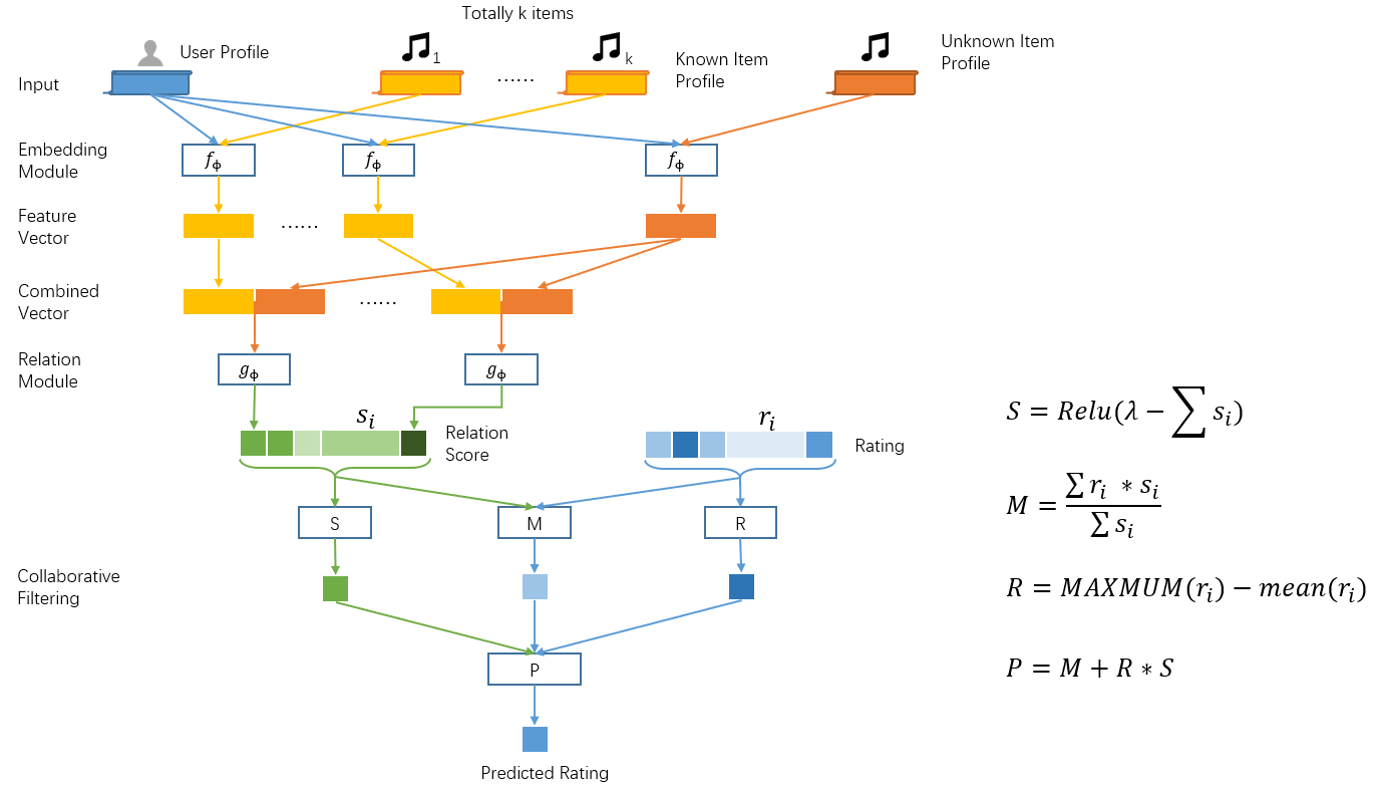
\includegraphics[width=15cm]  {MusicRecomSurvey/pics/model.PNG}}    
\caption{\label{4} 模型结构图}      
\end{figure}

\paragraph{输入}
模型的输入主要包含两部分:一部分是特征信息,包含目标用户的特征信息、已经评分的$k$首歌曲的特征信息以及目标歌曲的特征信息。另一部分是评分信息,包含了目标用户对于$k$首已经评分歌曲的评分值。

\paragraph{Embedding Module}
由于我们获取的特征信息并不是形式化的向量值,所以需要对其进Embedding从而对于特征进行提取。而我们在这里的一个设计是将用户特征和音乐特征结合其来进行Embedding处理。因为我们认为不同的人对于音乐有不同的偏好,所以在提取特征时,如果只对于音乐特征进行特征提取和描述,则无法体现出不同用户对于这些音乐的交互特征。所以我们在进行特征提取时,就将两者的特征进行了整合。如图中$f_{\phi}$模块所示,其输入为目标用户的信息和音乐的信息,输出为对于两者进行组合和编码后,得到的向量化的用户评分行为的特征信息。这里可用的方法有很多种,可以使用AutoEncoder模型来完成特征提取,也可以使用其他的特征提取方法。

\paragraph{Relation Module}
在上一部分中,我们将数据集中关于用户和音乐的信息进行处理,得到了其高阶非线性特征向量作为输出。在下一部分的模型中,我们希望能通过这样的特征,给出用户对不同的音乐之间的评分相似性给出一个评价。我们首先将用户对于已评分歌曲的特征和目标未评分歌曲的特征进行组合,表示比较相关性的两个歌曲特征,之后通过比较相似性的模块$g_{\phi}$来给出两者之间的相似性,并通过归一化函数将其大小限定在0到1之间,最终得到一个$k$维的数值向量Relation Score。

\paragraph{协同过滤}
在上面的输出中,我们得到了用户对未知歌曲的评价,与一些已知歌曲评分的相似性。之后就可以借助协同过滤方法对于目标用户对目标歌曲的评分进行估计。同时,为了更好地对于用户的评分进行预测,我们对于传统的估计方式进行了改进,使其能够对于ICS的情况具有更好的普适性和准确度。
首先额外输入用户对于这些已评价歌曲的评分$Rating$,结合之前得到的$Relation Score$,可以求出参数$M$,即传统的协同过滤当中根据相似度进行加权平均之后的估计值。我们通过另外两项参数$S$和$R$来对这个估计值进行修正。
我们通过参数$S$来描述当前评分信息的“可依赖性”。我们首先设置了一个阈值$\lambda$,通过对于相似度进行求和,得到的值与该阈值进行比较。如果相似度足够高,以至于高于$\lambda$,则经过$Relu$函数后,得到的参数$S=0$,这就表明当前样本能够提供足够多的相似歌曲的评分信息,此时,给出的评分也是比较准确的。相反,如果相似度很低,则$S>0$,这就表明过去的评分歌曲与当前的目标歌曲之间相似度不高,不能过分依赖于这些评分数据
我们通过参数$R$对于用户过去的评分行为进行描述。如果用户在过去对于一些歌曲的评分都很高,则$R$值也较大,可以认为这名听众是“宽容的”,此时如果$S$也较大,则我们对于这个与之前评分数据不太相似的歌曲的评价也是较高的。相反如果其对于过去听到的音乐的评分较低,则$R$值较小,用户对过去听到的歌曲较为不满,所以我们更倾向于向用户推荐与过去歌曲不相似的歌曲,则此时$S$值越大,就表明这个歌曲与之前用户听过的歌曲越不相似,从而预估的评分也越高。
综上,通过这样的方法,我们能够得到一个对于得分的估计值。

\paragraph{输出与结果}
上面的过程最终为我们给出了一个评分的预测值,接下来我们可以根据用户对于多个歌曲的评分预测,选出评价最高的,作为用户的推荐结果。

\subsubsection{模型创新点}
\paragraph{用户推荐个性化}
在之前的文献综述过程中,我们了解到了Item-Based的协同过滤方法,但是我们在讨论过程中发现这一系列方案中,虽然可能考虑到了音乐在各方面的特征,但是对于不同的用户,其表现是相同的。但是这种情况确实是不合理的。所以我们希望能够通过联合用户和音乐的信息,共同进行特征的提取,这样,对于不同的人,相同的音乐的特征也将会是不同的,所以这里的特征包含了用户更加“个性化”的信息。这种“个性化”就体现在我们模型中Embedding Module对于用户信息和音乐信息进行联合的特征提取。

\paragraph{高阶特征提取}
在之前对于$Metric Learning$的文献调研中,我们发现其基本的想法是定义距离,在这里也可以理解为相似性,但是,进一步的研究发现这里定义的距离,本质上来看,仍然是线性的,低阶的距离。这样来看,我们虽然能够提取出高阶的特征,但是在相似度度量上仍然是通过低阶的方法来实现的。所以我们希望能真正用到这部分告诫特征。所以设计了$Relation Module$的结构,我们希望通过训练数据,使得我们的模型能够学到如何对于相似性进行判定,而这里的相似性就利用的是高阶非线性的方法求出的相似性。所以我们的模型能够更有效地利用我们提取出的高阶特征。

\paragraph{用户评分偏差的修正}
考虑这样一个场景:一个用户打了很多的低分。根据传统的协同过滤方法,我们建立相似度,根据其进行加权平均,最后无论相似与否,其分值都很低,所以推荐系统就接近退化于盲目地进行推荐。这样推荐出的歌曲有很多也是用户不感兴趣的,所以打出了更多的低分。这种情况下,用户的体验是不好的。但是,如果假定用户并不是故意打差评,那么我们认为出现多次的低分,推荐系统应该能够表现得更加“重要”,给出用户潜在的感兴趣的内容。所以我们给出了一个思路,就是推荐和之前低分音乐相似度低的音乐,从而减小推荐出不感兴趣内容的概率,改善用户的使用体验。





